\documentclass[aspectratio=169,11pt]{beamer}

\usetheme{Madrid}
\usecolortheme{whale}
\setbeamertemplate{navigation symbols}{}
\setbeamertemplate{footline}[frame number]

\usepackage[utf8]{inputenc}
\usepackage[T1]{fontenc}
\usepackage{booktabs}
\usepackage{xcolor}
\usepackage{hyperref}
\usepackage{listings}
\usepackage{tikz}
\usetikzlibrary{positioning}

\lstset{
    basicstyle=\ttfamily\scriptsize,
    breaklines=true,
    frame=single,
    backgroundcolor=\color{gray!10},
    keywordstyle=\color{blue!70},
    commentstyle=\color{green!50!black},
    stringstyle=\color{red!60},
    showstringspaces=false,
    tabsize=2
}

\definecolor{stepbg}{RGB}{232,245,233}
\definecolor{stepborder}{RGB}{76,175,80}
\definecolor{warnbg}{RGB}{255,243,224}
\definecolor{warnborder}{RGB}{255,152,0}
\definecolor{aibg}{RGB}{243,229,245}
\definecolor{aiborder}{RGB}{156,39,176}

\title[EECE5155 -- Hands-On 3]{IoT Dataset Analysis: Real Deployment Data}
\subtitle{Hands-On Session 3: Use AI to Code, Use Your Brain to Interpret}
\author{Eduardo Baena}
\date{Thursday, March 26, 2026}
\institute{Northeastern University\\EECE5155: Wireless Sensor Networks and IoT}

\begin{document}

\begin{frame}
    \titlepage
\end{frame}

%==============================================================================
\section{Why Analyze Before You Collect?}
%==============================================================================

\begin{frame}[shrink=5]{Real IoT Data Is Messy}
    \begin{columns}
        \column{0.55\textwidth}
        \textbf{What we find in real deployments:}
        \begin{itemize}
            \item Missing values (sensor disconnected, battery died)
            \item Outliers (electromagnetic interference, stuck readings)
            \item Sensor drift (calibration degrades over time)
            \item Irregular timestamps (network latency, clock drift)
            \item Duplicate readings (MQTT QoS retransmissions)
        \end{itemize}

        \vspace{0.15cm}
        \textbf{Why this matters for our MVPs:}
        \begin{itemize}
            \item We \textbf{will} encounter these issues with real hardware
            \item Our demo must handle them gracefully
            \item The final report must document data quality
        \end{itemize}

        \column{0.45\textwidth}
        \fcolorbox{aiborder}{aibg}{
        \begin{minipage}{0.9\textwidth}
            \vspace{0.1cm}
            \small
            \textbf{AI era context:}

            \vspace{0.1cm}
            Today's rules:
            \begin{enumerate}
                \item Use \textbf{any AI tool} (ChatGPT, Copilot, etc.) to generate code
                \item \textbf{You} write the interpretation
                \item AI cannot tell you: is that outlier real or noise? Should we interpolate or drop? Is drift a sensor problem or a real signal?
            \end{enumerate}

            \vspace{0.1cm}
            Only \textbf{you} know the physical context.
            \vspace{0.1cm}
        \end{minipage}
        }

        \vspace{0.1cm}
        \begin{alertblock}{Grading: 40\% code works, 60\% interpretation}
            \small
            The code is the easy part. The interpretation is the engineering.
        \end{alertblock}
    \end{columns}
\end{frame}

\begin{frame}[shrink=5]{The Intel Berkeley Research Lab Deployment}
    \begin{columns}
        \column{0.55\textwidth}
        \textbf{The story behind the data:}

        \vspace{0.15cm}
        \begin{itemize}
            \item \textbf{Where:} UC Berkeley computer science lab, 2004
            \item \textbf{What:} 54 Mica2Dot wireless sensor nodes
            \item \textbf{Sensors:} temperature, humidity, light, battery voltage
            \item \textbf{Duration:} 38 days continuous operation
            \item \textbf{Result:} 2.3 million readings
            \item \textbf{Sampling:} $\sim$31 seconds per reading per node
        \end{itemize}

        \vspace{0.15cm}
        \textbf{Why this dataset matters:}
        \begin{itemize}
            \item One of the \textbf{most cited} IoT datasets in research
            \item Real deployment = real problems (sensors died, data corrupted)
            \item Same scale as our MVPs: tens of sensors, weeks of data
        \end{itemize}

        \column{0.45\textwidth}
        \fcolorbox{stepborder}{stepbg}{
        \begin{minipage}{0.9\textwidth}
            \vspace{0.1cm}
            \small
            \textbf{Deployment facts:}

            \vspace{0.1cm}
            \begin{tabular}{ll}
                Nodes      & 54 Mica2Dot \\
                Radio      & TinyOS / 916 MHz \\
                MCU        & ATmega128L \\
                RAM        & 4 KB \\
                Sampling   & $\sim$31 sec \\
                Battery    & 2$\times$AA cells \\
                Failures   & $>$10 nodes died \\
            \end{tabular}
            \vspace{0.1cm}
        \end{minipage}
        }

        \vspace{0.15cm}
        \begin{alertblock}{\small Context for today}
            \small
            We analyze this data as if we just inherited someone else's deployment. No access to the lab. Only the CSV.
        \end{alertblock}
    \end{columns}
\end{frame}

\begin{frame}[shrink=5]{IoT Data Lifecycle: Where Things Go Wrong}
    \begin{center}
    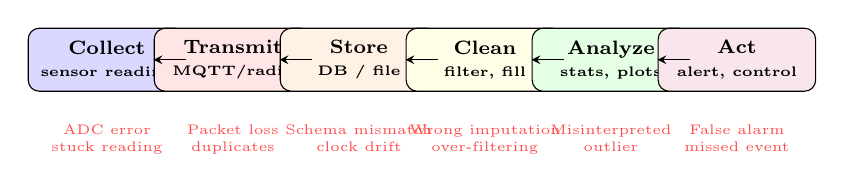
\begin{tikzpicture}[>=stealth, node distance=1.6cm,
        stage/.style={rectangle, rounded corners, draw, minimum width=2cm,
                      minimum height=0.8cm, font=\scriptsize\bfseries, align=center}]
        \node[stage, fill=blue!15]   (collect)   {Collect\\\tiny sensor reading};
        \node[stage, fill=red!10, right of=collect]    (transmit)  {Transmit\\\tiny MQTT/radio};
        \node[stage, fill=orange!10, right of=transmit] (store)     {Store\\\tiny DB / file};
        \node[stage, fill=yellow!10, right of=store]    (clean)     {Clean\\\tiny filter, fill};
        \node[stage, fill=green!10, right of=clean]     (analyze)   {Analyze\\\tiny stats, plots};
        \node[stage, fill=purple!10, right of=analyze]  (act)       {Act\\\tiny alert, control};

        \draw[->] (collect) -- (transmit);
        \draw[->] (transmit) -- (store);
        \draw[->] (store) -- (clean);
        \draw[->] (clean) -- (analyze);
        \draw[->] (analyze) -- (act);

        \node[below=0.3cm of collect, font=\tiny, text=red!70, align=center] {ADC error\\stuck reading};
        \node[below=0.3cm of transmit, font=\tiny, text=red!70, align=center] {Packet loss\\duplicates};
        \node[below=0.3cm of store, font=\tiny, text=red!70, align=center] {Schema mismatch\\clock drift};
        \node[below=0.3cm of clean, font=\tiny, text=red!70, align=center] {Wrong imputation\\over-filtering};
        \node[below=0.3cm of analyze, font=\tiny, text=red!70, align=center] {Misinterpreted\\outlier};
        \node[below=0.3cm of act, font=\tiny, text=red!70, align=center] {False alarm\\missed event};
    \end{tikzpicture}
    \end{center}

    \vspace{0.1cm}
    \begin{columns}
        \column{0.5\textwidth}
        \textbf{Key insight:} errors compound downstream.
        \begin{itemize}
            \item A stuck ADC at collection $\rightarrow$ looks like a real outlier at analysis $\rightarrow$ triggers a false alarm at action
            \item \textbf{Today:} we learn to catch problems at the analysis stage before they reach the action stage
        \end{itemize}

        \column{0.5\textwidth}
        \fcolorbox{warnborder}{warnbg}{
        \begin{minipage}{0.9\textwidth}
            \vspace{0.1cm}
            \small
            \textbf{For our MVPs:}
            \begin{itemize}
                \item Mon: we built Collect + Transmit
                \item Wed: we built Store + Act
                \item Today: we learn Clean + Analyze
                \item \textbf{Full pipeline ready for hardware}
            \end{itemize}
            \vspace{0.1cm}
        \end{minipage}
        }
    \end{columns}
\end{frame}

\begin{frame}[shrink=8]{Real-World IoT Data Failures}
    \textbf{When data quality is ignored, bad things happen:}

    \vspace{0.2cm}
    \begin{columns}
        \column{0.33\textwidth}
        \fcolorbox{warnborder}{warnbg}{
        \begin{minipage}{0.9\textwidth}
            \vspace{0.1cm}
            \centering\scriptsize
            \textbf{Nest Thermostat (2016)}

            \vspace{0.1cm}
            \raggedright
            Firmware 5.1.3 drained batteries overnight. Homes dropped to 5\textdegree{}C. Users woke up to no heat.

            \vspace{0.1cm}
            \textbf{Root cause:} bug in software update caused the thermostat to become unresponsive. Battery voltage data was misinterpreted.

            \vspace{0.1cm}
            \textit{Lesson: test data pipelines after firmware updates.}

            \vspace{0.1cm}
            \textbf{Source:} \href{https://www.theregister.com/2016/01/14/nest_foul_up/}{The Register}
            \vspace{0.1cm}
        \end{minipage}
        }

        \column{0.33\textwidth}
        \fcolorbox{aiborder}{aibg}{
        \begin{minipage}{0.9\textwidth}
            \vspace{0.1cm}
            \centering\scriptsize
            \textbf{Air Quality Sensors (Helsinki)}

            \vspace{0.1cm}
            \raggedright
            25 low-cost sensors deployed across Helsinki. Cross-sensitivity between O$_3$ and NO$_2$, plus humidity interference, caused systematic errors.

            \vspace{0.1cm}
            \textbf{Root cause:} electrochemical sensors respond to multiple gases. Humidity changes readings by 10--20\%.

            \vspace{0.1cm}
            \textit{Lesson: cross-validate with reference sensors.}

            \vspace{0.1cm}
            \textbf{Source:} \href{https://www.frontiersin.org/journals/environmental-science/articles/10.3389/fenvs.2021.719567/full}{Frontiers 2021}
            \vspace{0.1cm}
        \end{minipage}
        }

        \column{0.33\textwidth}
        \fcolorbox{stepborder}{stepbg}{
        \begin{minipage}{0.9\textwidth}
            \vspace{0.1cm}
            \centering\scriptsize
            \textbf{Intel Lab Dataset (Today)}

            \vspace{0.1cm}
            \raggedright
            54 sensors deployed across a UC Berkeley computer science lab for 38 days (2004).

            \vspace{0.1cm}
            Measured: temperature, humidity, light, battery voltage.

            \vspace{0.1cm}
            Total: 2.3 million readings.

            \vspace{0.1cm}
            \textbf{Source:} \href{https://db.csail.mit.edu/labdata/labdata.html}{MIT CSAIL}
            \vspace{0.1cm}
        \end{minipage}
        }
    \end{columns}

    \vspace{0.15cm}
    \begin{block}{Common thread}
        In every case, the \textbf{data was available} to detect the problem. The issue was that nobody analyzed it properly. That is what we practice today.
    \end{block}
\end{frame}

%==============================================================================
\section{Setup}
%==============================================================================

\begin{frame}[fragile]{Step 0: Download the Dataset (5 min)}
    \textbf{Intel Berkeley Research Lab Sensors (2004)}\\
    {\small 54 sensors, temperature + humidity + light + voltage, 2.3M readings over 38 days.}

    \vspace{0.2cm}
    \begin{lstlisting}[language=bash]
# Create working directory
mkdir -p ~/iot-dataset-lab && cd ~/iot-dataset-lab

# Download the Intel Lab dataset
curl -L -o data.txt.gz \
  "https://db.csail.mit.edu/labdata/data.txt.gz"
gunzip data.txt.gz
    \end{lstlisting}

    \vspace{0.1cm}
    \begin{lstlisting}[language=python]
import pandas as pd

cols = ['date','time','epoch','moteid','temperature',
        'humidity','light','voltage']
df = pd.read_csv('data.txt', sep=r'\s+', names=cols,
                  na_values=[''])
df['timestamp'] = pd.to_datetime(df['date'] + ' ' + df['time'],
                                 errors='coerce')
print(f"Shape: {df.shape}")
print(df.head())
print(f"\nMissing values:\n{df.isnull().sum()}")
    \end{lstlisting}

    \fcolorbox{stepborder}{stepbg}{
    \begin{minipage}{0.95\textwidth}
        \small
        \textbf{Resources:}
        \begin{itemize}
            \item \textbf{Colab notebook:} \url{https://shorturl.at/7lvsf}
            \item \textbf{Alt dataset:} \url{https://github.com/chrico03/IoT-Timeseries-Datasets}
        \end{itemize}
    \end{minipage}
    }
\end{frame}

%==============================================================================
\section{Exercise 1: Data Quality Audit}
%==============================================================================

\begin{frame}[shrink=5]{Exercise 1: Data Quality Audit (20 min)}
    \begin{columns}
        \column{0.55\textwidth}
        \textbf{Use AI to write code that answers these questions:}

        \vspace{0.15cm}
        \begin{enumerate}
            \item How many readings did each of the 54 sensors produce? Which sensors have far fewer readings than others?

            \item How many missing values (NaN) does each sensor have for temperature and humidity?

            \item Plot a histogram of \textbf{all} temperature readings. What do the tails look like?

            \item Plot temperature over time for motes 1, 2, 15, and 49 on the same chart.
        \end{enumerate}

        \vspace{0.1cm}
        \fcolorbox{aiborder}{aibg}{
        \begin{minipage}{0.9\textwidth}
            \scriptsize
            \vspace{0.05cm}
            \textbf{Suggested AI prompt:} ``I have a pandas DataFrame \texttt{df} with columns: moteid, temperature, humidity, timestamp. Write code to count readings per sensor and show the distribution statistics.''
            \vspace{0.05cm}
        \end{minipage}
        }

        \column{0.45\textwidth}
        \textbf{YOU write the interpretation:}

        \vspace{0.15cm}
        \fcolorbox{warnborder}{warnbg}{
        \begin{minipage}{0.9\textwidth}
            \vspace{0.1cm}
            \small
            In a markdown cell, answer:
            \begin{itemize}
                \item Which sensor IDs died early? \textbf{Why} might a sensor die? (battery, connectivity, physical damage?)
                \item Are missing values random or clustered in time? What does each pattern mean?
                \item The histogram shows readings $>$40\textdegree{}C in an indoor lab. Is that physically possible? What caused it?
                \item Mote 49 stops reporting. \textbf{When} did it die? How can you tell?
            \end{itemize}
            \vspace{0.1cm}
        \end{minipage}
        }

        \vspace{0.1cm}
        \begin{alertblock}{\small Save plot as \texttt{data\_quality.png}}
        \end{alertblock}
    \end{columns}
\end{frame}

%==============================================================================
\section{Exercise 2: Sensor Comparison}
%==============================================================================

\begin{frame}[shrink=5]{Exercise 2: Compare Sensors (20 min)}
    \begin{columns}
        \column{0.55\textwidth}
        \textbf{Use AI to write code that answers:}

        \vspace{0.15cm}
        \begin{enumerate}
            \item Pick sensors 1, 2, 33, and 34. Resample each to 5-minute averages and plot temperature over time on the same chart.

            \item Compute the \textbf{correlation matrix} between these four sensors.

            \item At each timestamp, compute the \textbf{spread} (max $-$ min). What is the worst-case spread?
        \end{enumerate}

        \vspace{0.1cm}
        \fcolorbox{aiborder}{aibg}{
        \begin{minipage}{0.9\textwidth}
            \scriptsize
            \vspace{0.05cm}
            \textbf{Hint for AI:} ``Resample to 5-min means, create a pivot table with sensors as columns, compute \texttt{.corr()} and max spread.''
            \vspace{0.05cm}
        \end{minipage}
        }

        \vspace{0.1cm}
        \begin{alertblock}{\small Save plot as \texttt{sensor\_comparison.png}}
        \end{alertblock}

        \column{0.45\textwidth}
        \textbf{YOU write the interpretation:}

        \vspace{0.15cm}
        \fcolorbox{warnborder}{warnbg}{
        \begin{minipage}{0.9\textwidth}
            \vspace{0.1cm}
            \small
            In a markdown cell, answer:
            \begin{itemize}
                \item Do the four sensors track each other? Where do they diverge?
                \item If one sensor reads 1.5\textdegree{}C higher consistently, give \textbf{two possible physical explanations}.
                \item Your PES says $\pm$0.5\textdegree{}C. Is that achievable given what you see here? What would you need to verify it?
                \item How would you decide which sensor to trust if they disagree?
            \end{itemize}
            \vspace{0.1cm}
        \end{minipage}
        }

        \vspace{0.1cm}
        \fcolorbox{stepborder}{stepbg}{
        \begin{minipage}{0.9\textwidth}
            \scriptsize
            \vspace{0.05cm}
            \textbf{Expected:} correlations $>$ 0.9 for nearby sensors. Max spread $\sim$120\textdegree{}C (outliers!) but median $<$1\textdegree{}C.
            \vspace{0.05cm}
        \end{minipage}
        }
    \end{columns}
\end{frame}

%==============================================================================
\section{Exercise 3: Anomaly Detection}
%==============================================================================

\begin{frame}[shrink=5]{Exercise 3: Anomaly Detection (15 min)}
    \begin{columns}
        \column{0.55\textwidth}
        \textbf{Use AI to write code for two anomaly detectors on Mote~1:}

        \vspace{0.15cm}
        \begin{enumerate}
            \item \textbf{Fixed thresholds:} Flag any temperature outside 15--35\textdegree{}C. Count how many anomalies.

            \item \textbf{Rolling z-score:} Compute a 1-hour rolling mean and std. Flag any reading with $|z| > 3$. Count anomalies.

            \item Plot both on the same chart: normal readings in blue, fixed-threshold anomalies in red, statistical anomalies in green.
        \end{enumerate}

        \vspace{0.1cm}
        \fcolorbox{aiborder}{aibg}{
        \begin{minipage}{0.9\textwidth}
            \scriptsize
            \vspace{0.05cm}
            \textbf{Hint for AI:} ``Filter Mote 1 temperature. Method 1: flag outside [15,35]. Method 2: rolling('1h').mean/std, flag abs(z)$>$3. Plot both on same axes.''
            \vspace{0.05cm}
        \end{minipage}
        }

        \vspace{0.1cm}
        \begin{alertblock}{\small Save plot as \texttt{anomalies.png}}
        \end{alertblock}

        \column{0.45\textwidth}
        \textbf{YOU write the interpretation:}

        \vspace{0.15cm}
        \fcolorbox{warnborder}{warnbg}{
        \begin{minipage}{0.9\textwidth}
            \vspace{0.1cm}
            \small
            In a markdown cell, answer:
            \begin{itemize}
                \item How many anomalies did each method find? Why are the numbers so different?
                \item Give an example of an anomaly caught by fixed threshold but \textbf{not} by z-score. Why?
                \item Give an example caught by z-score but \textbf{not} by fixed threshold. Why?
                \item For \textbf{your} MVP project: which method would you use for safety alerts? Which for drift detection?
            \end{itemize}
            \vspace{0.1cm}
        \end{minipage}
        }

        \vspace{0.1cm}
        \fcolorbox{stepborder}{stepbg}{
        \begin{minipage}{0.9\textwidth}
            \scriptsize
            \vspace{0.05cm}
            \textbf{Expected:} fixed threshold finds $\sim$6700, z-score finds $\sim$500. Only $\sim$10 overlap. Think about why.
            \vspace{0.05cm}
        \end{minipage}
        }
    \end{columns}
\end{frame}

\begin{frame}[shrink=5]{Class Discussion: What Did We Learn?}
    \begin{columns}
        \column{0.5\textwidth}
        \textbf{Let's compare results (5 min):}

        \vspace{0.15cm}
        \begin{enumerate}
            \item \textbf{Exercise 1:} How many sensors died? Did everyone get the same count? Why might counts differ?

            \item \textbf{Exercise 2:} What correlations did we get? Anyone find a sensor pair with low correlation?

            \item \textbf{Exercise 3:} How many anomalies by each method? Why the huge difference between fixed and statistical?
        \end{enumerate}

        \vspace{0.1cm}
        \textbf{Discussion question:}

        \vspace{0.1cm}
        \textit{``A reading of 38\textdegree{}C appears once at 3 AM in the lab. Is it real or noise? How do you decide?''}

        \column{0.5\textwidth}
        \textbf{Key takeaways:}

        \vspace{0.15cm}
        \begin{itemize}
            \item \textbf{18\% of the dataset} has temperature $>$40\textdegree{}C. If we used raw data without cleaning, our analysis would be garbage.

            \item \textbf{Nearby sensors correlate at 0.98+}. If one drops below 0.8, investigate it.

            \item \textbf{Fixed thresholds and z-scores find different anomalies.} Neither is complete alone. Use both.

            \item \textbf{Physical context is everything.} The same 35\textdegree{}C reading means ``normal'' outdoors and ``sensor error'' indoors.
        \end{itemize}

        \vspace{0.1cm}
        \fcolorbox{aiborder}{aibg}{
        \begin{minipage}{0.9\textwidth}
            \scriptsize
            \vspace{0.05cm}
            \textbf{AI can compute all of this.} But it cannot tell us whether 38\textdegree{}C at 3 AM is the HVAC shutting off or a stuck sensor. That is our job.
            \vspace{0.05cm}
        \end{minipage}
        }
    \end{columns}
\end{frame}

\begin{frame}[shrink=5]{Thinking Like an Anomaly Detective}
    \textbf{How do you know when something is ``wrong'' with your data?}

    \vspace{0.15cm}
    \begin{columns}
        \column{0.48\textwidth}
        \textbf{Ask these questions:}
        \begin{enumerate}
            \item \textbf{Is this physically possible?} \
                  45\textdegree{}C in a 22\textdegree{}C lab? No. \
                  35\textdegree{}C outdoors in July? Maybe.

            \item \textbf{Do nearby sensors agree?} \
                  If Mote 1 says 22\textdegree{}C and Mote 2 says 38\textdegree{}C at the same time, one is wrong.

            \item \textbf{Is this a sudden jump or gradual drift?} \
                  Sudden $\rightarrow$ sensor glitch or event. \
                  Gradual $\rightarrow$ calibration drift or battery dying.

            \item \textbf{Does it match a known pattern?} \
                  HVAC cycles, daily rhythms, weekly schedules.
        \end{enumerate}

        \column{0.48\textwidth}
        \textbf{Red flags in IoT data:}
        \vspace{0.1cm}

        \fcolorbox{warnborder}{warnbg}{
        \begin{minipage}{0.95\textwidth}
            \vspace{0.1cm}
            \scriptsize
            \begin{itemize}
                \item Same value repeated 100+ times $\rightarrow$ stuck ADC
                \item Correlation drops suddenly $\rightarrow$ sensor degraded
                \item Missing data at same hour daily $\rightarrow$ scheduled reboot
                \item Values outside sensor spec $\rightarrow$ electrical noise
                \item Bimodal distribution $\rightarrow$ two different operating modes
            \end{itemize}
            \vspace{0.1cm}
        \end{minipage}
        }

        \vspace{0.15cm}
        \fcolorbox{aiborder}{aibg}{
        \begin{minipage}{0.95\textwidth}
            \vspace{0.1cm}
            \scriptsize
            \textbf{The key skill:} AI can compute z-scores and correlations. But only YOU can say ``this pattern looks like a dying battery because I've seen it before.'' That's engineering judgment.
            \vspace{0.1cm}
        \end{minipage}
        }
    \end{columns}
\end{frame}

\begin{frame}[shrink=5]{Homework: Apply to Other Datasets}
    \textbf{Now apply the same three exercises to one of these datasets:}

    \vspace{0.15cm}
    \footnotesize
    \begin{tabular}{p{3.2cm}p{4cm}p{2.3cm}p{2.5cm}}
        \toprule
        \textbf{Dataset} & \textbf{What it contains} & \textbf{Year} & \textbf{Good for} \\
        \midrule
        Google Smart Buildings & 6 years of temp, humidity, occupancy, energy from 3 buildings & 2024 & Real-world drift \\
        \midrule
        NAB Benchmark & 58 labeled time series with \textbf{known anomalies} & 2015 & Testing detectors \\
        \midrule
        ASHRAE Energy & Building HVAC + weather + energy, 20M rows & 2019 & Seasonal patterns \\
        \midrule
        UCI Air Quality & CO, NOx, benzene from urban sensors & 2016 & Multivariate fusion \\
        \midrule
        Kaggle Smart Home & Appliance energy + temperature & 2018 & Home automation \\
        \bottomrule
    \end{tabular}
    \normalsize

    \vspace{0.15cm}
    \begin{columns}
        \column{0.48\textwidth}
        \fcolorbox{stepborder}{stepbg}{
        \begin{minipage}{0.9\textwidth}
            \vspace{0.1cm}
            \scriptsize
            \textbf{Google Smart Buildings Dataset} — \href{https://www.tensorflow.org/datasets/catalog/smart_buildings}{TensorFlow Datasets} \\
            Real data from 2017–2023. Includes occupancy, which Intel Lab lacks. Perfect for testing ``does temperature spike when room is empty?''
            \vspace{0.1cm}
        \end{minipage}
        }

        \column{0.48\textwidth}
        \fcolorbox{warnborder}{warnbg}{
        \begin{minipage}{0.9\textwidth}
            \vspace{0.1cm}
            \scriptsize
            \textbf{NAB (Numenta Anomaly Benchmark)} — \href{https://github.com/numenta/NAB}{GitHub} \\
            The only dataset with \textbf{labeled anomalies}. You can test your detector and know if it caught the real anomalies. 50+ time series from AWS, traffic, ads.
            \vspace{0.1cm}
        \end{minipage}
        }
    \end{columns}

    \vspace{0.1cm}
    \fcolorbox{aiborder}{aibg}{
    \begin{minipage}{0.95\textwidth}
        \vspace{0.1cm}
        \small
        \textbf{Deliverable:} Submit a LaTeX report with the same three sections (quality audit, sensor comparison, anomaly detection) for your chosen dataset. Use the template from the repo.
        \vspace{0.1cm}
    \end{minipage}
    }
\end{frame}

%==============================================================================
\section{Wrap-Up}
%==============================================================================

\begin{frame}[shrink=5]{Deliverables + What We Built This Week}
    \begin{columns}
        \column{0.5\textwidth}
        \textbf{Submit on Canvas:}

        \vspace{0.15cm}
        \begin{enumerate}
            \item \textbf{LaTeX report} (use \texttt{dataset\_report\_template.tex}):
            \begin{itemize}
                \item Fill in results + interpretation for each exercise
                \item Compile to PDF
            \end{itemize}
            \item \textbf{3 plots} as PNG (embedded in report)
            \item \textbf{Jupyter notebook} (.ipynb) with your code
        \end{enumerate}

        \vspace{0.15cm}
        \fcolorbox{aiborder}{aibg}{
        \begin{minipage}{0.9\textwidth}
            \scriptsize
            \vspace{0.05cm}
            \textbf{Grading:} 40\% code runs and produces correct output. 60\% quality of written interpretation in the LaTeX report. AI-generated interpretations = 0.
            \vspace{0.05cm}
        \end{minipage}
        }

        \column{0.5\textwidth}
        \textbf{Complete week summary:}

        \vspace{0.1cm}
        \begin{tabular}{llll}
            \toprule
            \textbf{Session} & \textbf{Skill} & \textbf{Artifact} \\
            \midrule
            Mon 23 & Firmware & Wokwi project \\
            Wed 25 & Automation & Node-RED flow \\
            \textbf{Thu 26} & \textbf{Data analysis} & \textbf{Notebook} \\
            \bottomrule
        \end{tabular}

        \vspace{0.2cm}
        \fcolorbox{stepborder}{stepbg}{
        \begin{minipage}{0.9\textwidth}
            \small
            \vspace{0.05cm}
            \textbf{Monday Mar 30:} Bring laptop + BOM printout. We assemble hardware and flash firmware onto the real ESP32.
            \vspace{0.05cm}
        \end{minipage}
        }

        \vspace{0.15cm}
        \textbf{Mon 30+: Hardware arrives. We are ready.}
    \end{columns}
\end{frame}

\end{document}
